\section{Metodologia de trabalho} % (fold)
\label{sec:contribuindo_com_plataformas_abertas}

Um dos objetivos deste trabalho era contribuir com uma aplicação \textit{open-souce} disponível na plataforma \href{http://github.com}{GitHub}\footnote{Disponível em \url{http://github.com}.}. Na próxima seção será apresentada a forma como tais contribuições foram realizadas. Devido ao fato do repositório do {\code APT} estar armazenado no GitHub, a terminologia apresentada estará em maior conformidade com esta plataforma, porém o conceito de \textit{pull-request} ou  \textit{merge-request} é amplamente utilizado em outras plataformas, como \href{https://bitbucket.org/}{Bitbucket}\footnote{Disponível em \url{https://bitbucket.org}.}, \href{https://gitlab.com/}{GitLab}\footnote{Disponível em \url{http://gitlab.com}.} ou até mesmo \href{http://sourceforge.net/}{SourceForge}\footnote{Disponível em \url{http://sourceforge.net}.}.


\subsection*{Mantendo uma cópia} % (fold)
\label{sub:mantendo_uma_copia_sua}


Normalmente não temos autorização pra alterar as informações de outra pessoa sem seu o consentimento. Da mesma forma  acontece com os repositórios {\code git}. Assim, um dos primeiros passos para começar a contribuir com uma ferramenta \textit{open-source} é fazer uma cópia dela em seu repositório. Essa cópia pode ser feita basicamente de duas formas, no intuito de preservar os autores das modificações anteriores:

\begin{description}
	\item [\textit{Fork}]: O termo é amplamente utilizado quando queremos fazer uma copia de um repositório para a nossa conta em uma mesma plataforma. Normalmente este passo é realizado via interface gráfica, ainda no navegador. Na \autoref{fig:github_fork} é possível observar o botão no canto superior direito que permite realizar um \textit{fork} do repositório desejado.

	\begin{figure}[h]
	  \centering
		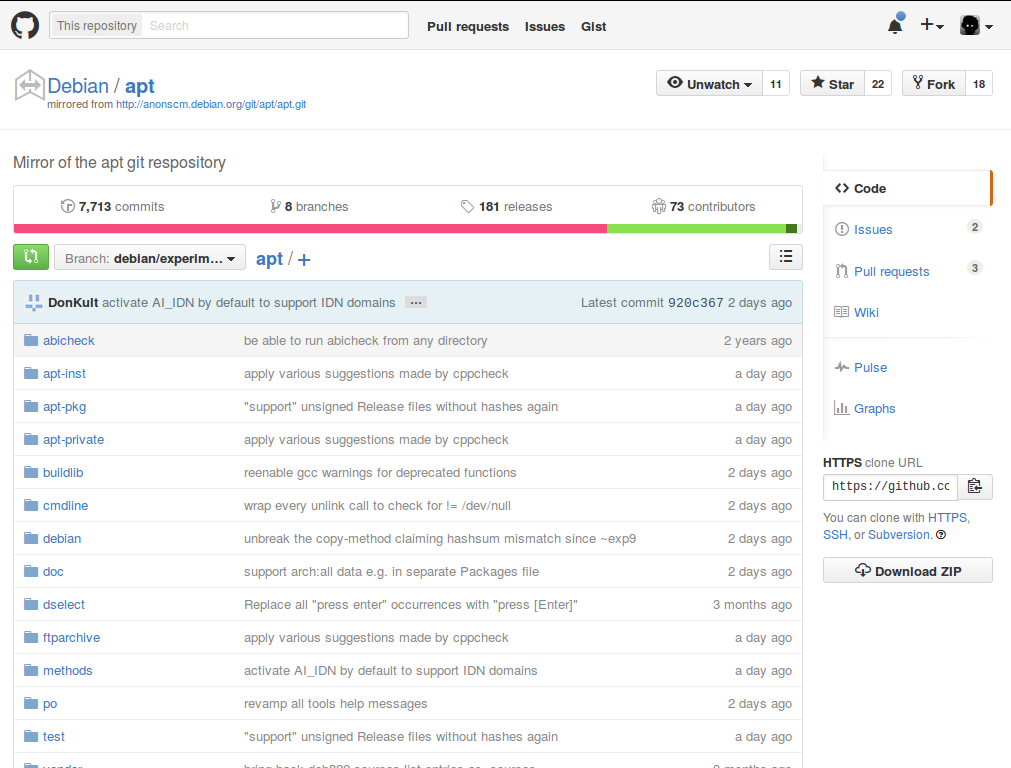
\includegraphics[width=0.90\textwidth]{figuras/fork}
	  \caption{Visão de um repositório do \textit{GitHub}, com destaque no botão que permite criar um \textit{fork} do projeto}
	  \label{fig:github_fork}
	\end{figure}

	\item [\textit{Adicionando \textit{remote}}]: Quando desejamos realizar uma cópia do repositório em uma plataforma distinta da original, a forma mais simples de proceder é clonando o repositório e incluindo nele um novo \textit{remote} para a nova plataforma. O \textit{remote} é o \textit{link} do repositório utilizado para a transmissão das alterações. Ele pode oferecer uma conexão {\code hhtps} ou {\code ssh}. Assim conseguimos trabalhar com a mesma árvore de \textit{commits} do repositório original, mantendo os créditos e alterações originais.
\end{description}
% subsection mantendo_uma_copia_sua (end)

\subsection*{Evoluindo o código} % (fold)
\label{sub:evoluindo_o_c_digo}

Nesto ponto de contribuição, o contribuinte desenvolve o código de acordo com o processo de produção escolhido. O código estará versionado em um repositório pessoal e o usuário possuirá todos os direitos administrativos deste repositório. Obviamente, caso a contribuição esteja sendo feita à uma aplicação grande e com muitos contribuidores, é importante se manter sincronizado com o código original, para evitar que o retorno da contribuição não seja tão trabalhoso para o revisor, além de evitar situações de conflito.
% subsection evoluindo_o_c_digo (end)

\subsection*{Retornando sua contribuição} % (fold)
\label{sub:retornando_sua_contribui_o}

Quando se decidido que a contribuição atinge um ponto aceitável para ser incorporada ao código original, é o momento de se realizar o \textit{pull-request}\footnote{Ou \textit{merge-request} dependendo da plataforma de desenvolvimento.}. Uma contribuição é interessante quando possui as seguintes características:


\begin{itemize}
	\item É uma significativa e relevante evolução de código mantendo os padrões de guia de estilo definido pelo desenvolvedor original/linguagem;
	\item Adiciona ou atende os testes para a evolução de código proposto;
	\item Traz a documentação da \textit{feature} implementada ou atualiza a documentação para contemplar as modificações sugeridas.
\end{itemize}
% subsection retornando_sua_contribui_o (end)

Submetida a contribuição, é dever do mantenedor do repositório original revisar o código e decidir se deve ou não aceitá-la.


\subsection*{Testando} % (fold)
\label{sub:testando}

É desejável, no desenvolvimento de software, existir um conjunto de testes unitários a cada evolução de código, a fim de validar as funcionalidades existentes ou adicionadas. No projeto abordado neste trabalho, em especial, há testes utilizado o \href{https://github.com/google/googletest}{Google C++ Testing Framework}\footnote{Disponível em \url{https://github.com/google/googletest}.} (Google Test), um \textit{framework} desenvolvido pela Google para testes. Ele tem suporte para um conjunto de assertivas pré-definidas e definidas pelo usuário, tornando-se uma das melhores ferramentas para a escrita de conjuntos de testes para C/C++ hoje disponíveis.

Outra categoria de testes se refere aos testes de integração. Neste trabalho em especial estará sendo utilizado um \textit{shell script} que oferece diversas funcionalidades para a criação dos testes de integração. Os testes de integração são utilizados no {\code APT} como testes caixa preta, a fim de verificar as funcionalidades em cenários de testes.

Os testes de integração tem maior prioridade que os unitários no APT, e podemos observar isso pela quantidade de testes em cada um deles. Nos testes unitários temos 20 casos de teste, totalizando 78 testes. Já nos testes de integração temos um conjunto de 199 cenários de testes, em um total de 24.976 testes\footnote{Dados relativos a \textit{build} \#219 do \href{https://travis-ci.org/Debian/apt/builds/}{Travis-CI}, disponível em \url{https://travis-ci.org/Debian/apt/builds/}.}.


\begin{lstlisting}[language=C++,label=gtestexample,caption={Teste de validação de armazenamento de parâmetros}]
TEST(CommandLineTest,SaveInConfig)
{
   EXPECT_CMD("apt-get install -sf",
	 "apt-get", "install", "-sf");
   EXPECT_CMD("apt-cache -s apt -so Debug::test=Test",
	 "apt-cache", "-s", "apt", "-so", "Debug::test=Test");
   EXPECT_CMD("apt-cache -s apt -so Debug::test=\"Das ist ein Test\"",
	 "apt-cache", "-s", "apt", "-so", "Debug::test=Das ist ein Test");
   EXPECT_CMD("apt-cache -s apt --hallo test=1.0",
	 "apt-cache", "-s", "apt", "--hallo", "test=1.0");
}
\end{lstlisting}

Um exemplo de teste unitário realizado é a validação do armazenamento dos parâmetros nas chamadas, como pode ser observado no \autoref{gtestexample}. Já testes de integração possuem um comparativo entre uma chamada e sua saída, como pode ser observado no \autoref{integrationtesteexample}.

\begin{lstlisting}[language=Bash,label=integrationtesteexample,caption={Teste de verificação de saída para busca}]
# without op progress
testsuccessequal "foo/unstable 1.0 all
  $DESCR
" apt search -qq xxyyzz
\end{lstlisting}

% subsection testando (end)
% section contribuindo_com_plataformas_abertas (end)


\section{Coleta de Dados} % (fold)
\label{cha:coleta_de_dados}

\subsection*{Tempo} % (fold)
\label{sec:tempo}

A coleta de tempo de performance de um software é uma tarefa árdua. A estimativa de tempo depende das otimizações que o compilador pode vir a fazer para a arquitetura, memória disponível, aplicativos rodando em \textit{background}, temperatura do hardware, etc. No intuito de simplificar o processo de estimativa de tempo, foi utilizado a mediana de uma série de execuções da aplicação. Segundo \citeonline{dolan2002benchmarking}, esta solução usando a mediana de uma série tem uma chance elevada de que o ponto selecionado melhor represente o comportamento padrão da sequência. Assim sendo, o \autoref{scriptods} foi uma solução desenvolvida para deixar a maquina dedicada para a aquisição de dados.

Para o funcionamento do \textit{script}, as variáveis {\code MAX} e {\code \_MAX\_THREADS} devem ser definidas com a quantidade de dados que se deseja coletar e a quantidade máxima de \textit{threads} que devem ser criadas para a chamada do processo, respectivamente. Usar uma quantidade superior à quantidade de \textit{cores}  da máquina pode produzir valores com baixa confiabilidade, visto a concorrência gerada pelas próprias \textit{threads}. Como parâmetros, foram escolhidos $150$ dados com $7$ \textit{threads}, deixando ao menos $1$ \textit{core} livre. Para maior dinamismo na coleta dos dados, o \textit{script} é responsável por realizar a troca das \textit{branchs} onde estão localizadas as possíveis soluções e a compilação e registro dos dados em uma planilha do \textit{LibreOffice Calc}. Assim, os algoritmos nunca são executados paralelamente, porém os dados serão coletado sob a demanda da $CPU$ na qual o \textit{script} é executado.

Para coletar o tempo de execução do algoritmo, o \autoref{libtime} foi desenvolvido a fim de ser usado como cronômetro. O algoritmo desenvolvido com o auxilio da biblioteca {\code Chrono}\footnote{Disponibilizada no {\code C++11} sob o \textit{namespace} {\code std::crono}.} permite a captura do intervalo de tempo com até $9$ casas decimais (nanosegundos), todavia foi utilizado a precisão de microssegundos ($10^ 6$) apenas, visto que o intervalo de nanosegundos não implicou em diferença significativa dos valores. Os métodos {\code begin()} e {\code end()} da classe são utilizados para pontuar os intervalos onde o tempo deve ser registrado. O resultado da medição pode ser obtido com o retorno do método {\code end()} ou com a chamada do {\code currenttime()}, dedicado apenas ao retorno deste valor.

\subsection*{Memória}

Para a coleta de memória, foi utilizado o {\code Valgrind}, com o auxílio da ferramenta {\code Massif}. Devido a criação da \textit{hash} ser feita de forma  algébrica e o método de \textit{KMP} utilizar um autômato finito determinístico, a repetição prévia das buscas com apenas $10$ amostras confirmavam a suspeita de não haver a variação do gasto de memória.

Para a execução da aplicação com o suporte ao {\code Valgrind} para análise do uso de memória, foi utilizado o comando:

\begin{lstlisting}[language=Bash,label=valgrind_call, numbers=none]
   $ valgrind --tool=massif  ./apt search pacote [--regex]
\end{lstlisting}
% section tempo (end)
% chapter coleta_de_dados (end)


\section{Ferramentas}

Para a realização desta contribuição as seguintes tecnologias estiveram envolvidas:

\begin{description}
	\item[Sublime-Text] Editor de texto.
	\item[Vim] Editor de texto.
	\item[Git] Sistema de controle de versão.
	\item[Make] Ferramenta de execução de comandos {\code bash}.
	\item[GCC] Compilador de C/C++.
	\item[Mint] Distribuição Linux baseada em Debian.
\end{description}

Os serviços das seguintes organizações também foram utilizados na produção deste trabalho:

\begin{description}
	\item[Github] Oferecem serviço de hospedagem de repositórios.
	\item[Travis CI] Oferecem serviço de Integração Continua.
\end{description}

Para desenvolvimento, foi utilizado uma maquina com as seguintes configurações:


\begin{description}
	\item[OS:] Mint 17.1 Rebecca
	\item[Kernel:] x86\_64 Linux 3.13.0-37-generic
	\item[CPU:] Intel Core i7 CPU 870 @ 2.934GHz
	\item[GPU:] GeForce GTX 465
	\item[RAM:] 12Gb
\end{description}


\section{Planejamento de contribuições} % (fold)
\label{sec:planejamento_de_contribui_es}

Como planejamento geral, foram definidas três grandes conjuntos de contribuições com o {\code APT}. A primeira contribuição tinha como objetivos a familiarização com o ambiente e com o time oficial de desenvolvimento. Para isso ela deveria conter uma contribuição simples, porém que viesse a oferecer maiores oportunidades posteriormente. A segunda contribuição tinha como objetivo a implantação dos algoritmos de \textit{string matching} exatos estudados sem descartar o modelo original de uso de expressões regulares para busca. Para a terceira e ultima contribuição o planejamento era a implantação do algoritmo de buscas inexatas em \textit{strings} para ser executado quando a pesquisa não retornasse nenhum resultado.

% section planejamento_de_contribui_es (end)

\section{Primeira contribuição} % (fold)
\label{sec:primeira_contribui_o}

Como tarefa, foi definido a implementação mínima de uma estrutura que permitisse um contexto de ordenação que pudesse ser definido pelo usuário. O intuito era oferecer as seguintes opções de ordenação:

\begin{description}
	\item [\textit{Alphabetic}] Ordenação padrão em ordem alfabética. Os pacotes são ordenados de acordo com seu nome.
	\item [\textit{Reverse Alphabetic}] Semelhante a ordenação alfabética, porém em ordem decrescente, ou seja, palavras que começam com {\code Z} são apresentadas antes das iniciadas com {\code A}.
	\item [\textit{Status}] Ordena os pacotes de acordo com as seguintes características, na ordem apresentada:
	\begin{enumerate}
		\item desinstalado,
		\item instalado e com possível atualização,
		\item instalado via pacote local,
		\item instalado e descartável (auto removível),
		\item instalado automaticamente,
		\item instalado,
		\item atualizável,
		\item com configuração residual
	\end{enumerate}
	\item [\textit{Version}] Ordena a saída de acordo com a versão do pacote.
\end{description}

\subsection*{Alteração da estrutura de dados} % (fold)
\label{sub:altera_o_da_estrutuda_de_dados}

Originalmente, os dados eram armazenados em um {\code std::map} padrão do {\code C++}, visto que essa estrutura não permite a duplicação de chaves e possui uma ordenação alfabética subjacente. Todavia, a alteração do algoritmo de ordenação de um {\code std::map} deve ser feita em sua declaração, o que inviabiliza a escolha da ordenação através de uma \textit{flag} passada como parâmetro de execução. Visto essa condição, a estrutura foi alterada para {\code std::vector}, por ser mais flexível quanto a sua forma de ordenação.

Naturalmente, a inserção de candidatos à saída do {\code APT} ocorre  em dois níveis. O primeiro nível ordena de acordo com os repositórios inseridos no {\code /etc/apt/sources.list} da distribuição. O segundo nível ordena cada bloco de pacotes recebidos de um repositório em ordem alfabética. Isso implica que apenas adicionar candidatos ao vetor resultaria em uma ordenação com baixa precisão, visto que a sequência de repositórios pode variar de usuário para usuário. Assim, a  troca de estrutura de dados de {\code std::map} para {\code std::vector} implica na necessidade de implementar o método de ordenação alfabética, nativamente implementado na estrutura {\code std::map}.

Um método para ordenação alfabética permite também ordenação alfabética reversa, visto que basta utilizar as referências do vetor inversas, ao invés da normais. Assim, foi necessário a escrita de três métodos, no total, para a primeira contribuição. O \autoref{choose_pr1} apresenta como a seleção de ordenação é realizada.


\begin{lstlisting}[language=C++,label=choose_pr1,caption={Tomada de decisão de ordenação}]
   switch(PackageInfo::getOrderByOption())
   {
      case PackageInfo::REVERSEALPHABETIC:
		 std::sort(outputVector.rbegin(), outputVector.rend(), OrderByAlphabetic);
		 break;
      case PackageInfo::STATUS:
			 std::sort(outputVector.begin(), outputVector.end(), OrderByStatus);
			 break;
      case PackageInfo::VERSION:
		 std::sort(outputVector.begin(), outputVector.end(), OrderByVersion);
		 break;
      default:
		 std::sort(outputVector.begin(), outputVector.end(),   OrderByAlphabetic);
		 break;
   }
\end{lstlisting}

A versão apresentada neste trabalho é o resultado de alguns \textit{feedback} sugeridos pelos mantenedores do projeto, em especial \href{https://github.com/DonKult}{David Kalnischkies}, o qual fez questão de pontuar detalhes na contribuição que poderiam ser melhorados ou questionados no processo de aceitação da contribuição.

% subsection altera_o_da_estrutuda_de_dados (end)

\subsection*{Testando alterações} % (fold)

Realizar uma contribuição que não ofereça testes ou atenda aos testes significa oferecer um trabalho sem garantias de funcionalidade. Desta forma, as contribuições realizadas neste trabalho também estiveram sempre acompanhadas de seus respectivos testes. O {\code APT} utiliza uma ferramenta de testes muito comum em $C++$, a \textit{Google Test}\footnote{Mais informações sobre a ferramenta podem ser obtidas em seu repositório oficial: \url{https://github.com/google/googletest}.}. Uma \textit{suíte} de testes é caracterizada pelo \textit{Google Test} como um arquivo contendo $N$ testes. Para manter o contexto, as condições da \textit{suíte} de testes devem ser definidas no início do arquivo.

\begin{lstlisting}[language=Bash,label=googletest_decl,caption={Declarações de instâncias para o teste}]
setupenvironment
configarchitecture "i386"

DESCR='Some description that has a unusual word xxyyzz and aabbcc and a UPPERCASE'
DESCR2='Some other description with the unusual aabbcc only'
DESCR3='Some package description'
DESCR4='an autogenerated dummy baz=0.1/installed'
insertpackage 'unstable' 'foo' 'all' '1.0' '' '' "$DESCR
 Long description of stuff and such, with lines
 .
 and paragraphs and everything."
insertpackage 'testing' 'bar' 'i386' '2.0' '' '' "$DESCR2"
insertpackage 'stable' 'package' 'all' '1.5' '' '' "$DESCR3"
insertinstalledpackage 'baz' 'all' '0.1'

setupaptarchive
\end{lstlisting}

Como apresentado no \autoref{googletest_decl}, algumas macros foram criadas pela equipe do {\code APT} para simplificar o processo de declaração de instâncias. Com estas instâncias declaradas, o contexto do teste é estabelecido e está pronto para rodar a \textit{suite} de testes. Os testes são basicamente cenários do estado do sistema, como pode ser observado no \autoref{gtest_foo}.

\begin{lstlisting}[language=Bash,label=gtest_foo,caption={Teste de busca pelo pacote \textit{foo}}]
# search name
testsuccessequal "foo/unstable 1.0 all
  $DESCR
" apt search -qq foo
\end{lstlisting}

Como estamos ordenando pacotes, era importante que se pudesse realizar uma busca por uma grande quantidade de pacotes. Uma das possibilidades que o {\code APT} possui hoje é a de se realizar buscas utilizando de expressões regulares. Unindo esta duas características, foi possível montar uma lista maior de pacotes e realizar uma busca por um termo genérico, a fim de obter como resultado toda a lista de pacotes. O exemplo o \autoref{buscacomregex} demostra este resultado, onde a busca é feita utilizando a \textit{regex} {\code \textbackslash w}, a fim de selecionar todos os pacotes que possuam pelo menos um caractere em seu nome.

\begin{lstlisting}[language=Bash,label=buscacomregex,caption={Busca com uso de expressão regular}]
# output is sorted by status
testsuccessequal "bar/testing 2.0 i386
  $DESCR2

foo/unstable 1.0 all
  $DESCR

package/stable 1.5 all
  $DESCR3

baz/now 0.1 all [installed,local]
  $DESCR4
" apt search --order-by status -qq "\\w"
\end{lstlisting}

\begin{figure}[h]
  \centering
	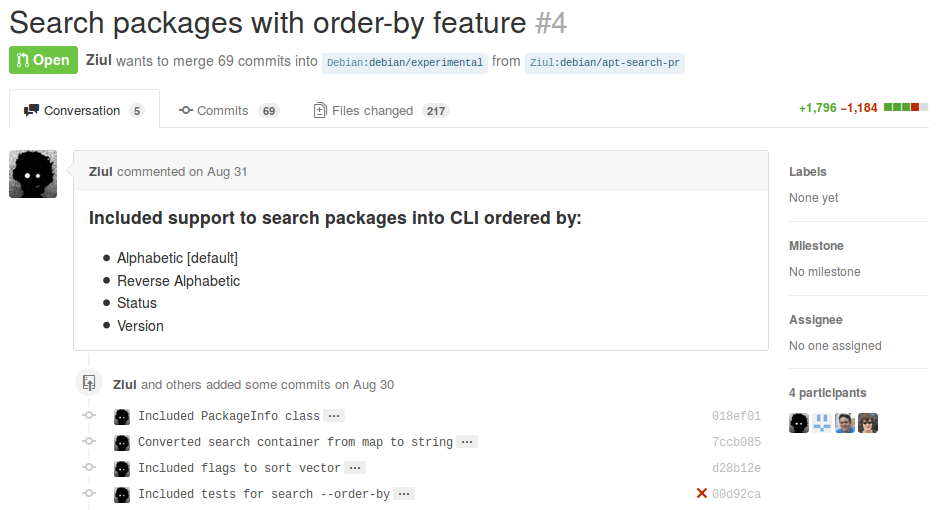
\includegraphics[width=0.75\textwidth]{figuras/pr1}
  \caption{Submissão do primeiro \textit{merge request}}
  \label{fig:pr1_travisnotok}
\end{figure}

A \autoref{fig:pr1_travisnotok} apresenta o resultado do \textit{merge request} e alguns dos \textit{commits} enviados, sendo que o último deles traz o resultado do \textit{Travis CI} apontando um problema na \textit{build} devido à falha em um dos testes de integração que verificam concorrência de download de arquivos.

% section primeira_contribui_o (end)


\section{Segunda contribuição} % (fold)
\label{sec:segunda_contribui_o}

O suporte a expressões regulares amplia a forma como a busca por pacotes pode ser efetuada, possibilitando uma maior gama de opções para desenvolvedores experientes. Todavia, deixar essa opção como padrão acarretaria em alguns pontos negativos:

\begin{description}
	\item [Alto consumo de memória:] Buscas com expressões regulares consomem cerca de $\Theta(2^n)$ de memória para uma expressão de tamanho $n$, ou $\Theta(n^2)$ para melhores casos, com hardware dedicado \cite{sidhu2001fast}.
	\item [Baixo desempenho:] Buscas com expressões regulares tem complexidade de execução $\Theta(n)$, sendo $n$ o tamanho da palavra a ser analisada.
\end{description}

Mesmo a busca com expressões regulares oferecendo um grande poder de busca, questiona-se se o custo que ela requer é aceitável. Vale lembrar que este trabalho visa ampliar a comodidade dos novos usuário Linux e as expressões regulares normalmente não são de conhecimento do usuário principiante. Considerando que este usuário não faria uso comumente, das funções {\code less}, {\code more} ou {\code grep} para refinar as buscas,  o uso de expressões regulares não será ampliado.

% Ora, se há a possibilidade de ganhar desempenho e gasto de memória mesmo ainda com busca exatas, há de se propor algoritmos para nos auxiliar com essas buscas.


Procurando por uma alternativa para a busca de pacotes que ofereça menor tempo de processamento e maior economia de memória, foram estudados dois algoritmos de \textit{string matching} exato apresentados na \autoref{sec:algoritimos_de_textit}; o \nameref{ssub:rabin_karp} e \nameref{ssub:knuth_morris_pratt_}. Para ambos os algoritmos foram criadas \textit{branchs} para seu desenvolvimento e testes de desempenho, fazendo de uso da rotina apresentada no \autoref{libtime} para mensurar o tempo gasto para na execução de cada um deles.

Diante dos resultados de tempo de execução obtidos com o algoritmo de \textit{Rabin-Karp}, a segunda contribuição foi planejada e executada. A \autoref{sec:segundo_pr} apresenta na integra o \textit{diff} da contribuição submetida para o repositório oficial.


A fim de manter a cobertura de teste das funcionalidades, testes foram elaborados para garantir que as buscas continuariam a ser realizadas com ou sem o uso da \textit{flag} que habilitava o uso de expressões regulares, como pode ser observado no \autoref{regextestscli}, onde um trecho dos testes da segunda submissão é apresentado.

\begin{lstlisting}[language=Bash,label=regextestscli,caption={Teste com e sem o uso de expressões regulares}]
# output is sorted by status
testequal "bar/testing 2.0 i386
  $DESCR2

foo/unstable 1.0 all
  $DESCR

package/stable 1.5 all
  $DESCR3

baz/now 0.1 all [installed,local]
  $DESCR4
" apt search --order-by status -qq "\\w" --regex

# output is sorted by Alphabetic (non case sense)
testequal "bar/testing 2.0 i386
  $DESCR2

baz/now 0.1 all [installed,local]
  $DESCR4
" apt search --order-by Alphabetic -qq ba
\end{lstlisting}

Finalizados os testes e a documentação das novas funcionalidades implementadas, foi realizado a submissão de \textit{merge request} ao repositório oficial do APT, a qual pode ser observada na \autoref{fig:pr2_travisok} e acompanhada em \url{https://github.com/Debian/apt/pull/8}.

\begin{figure}[h]
  \centering
	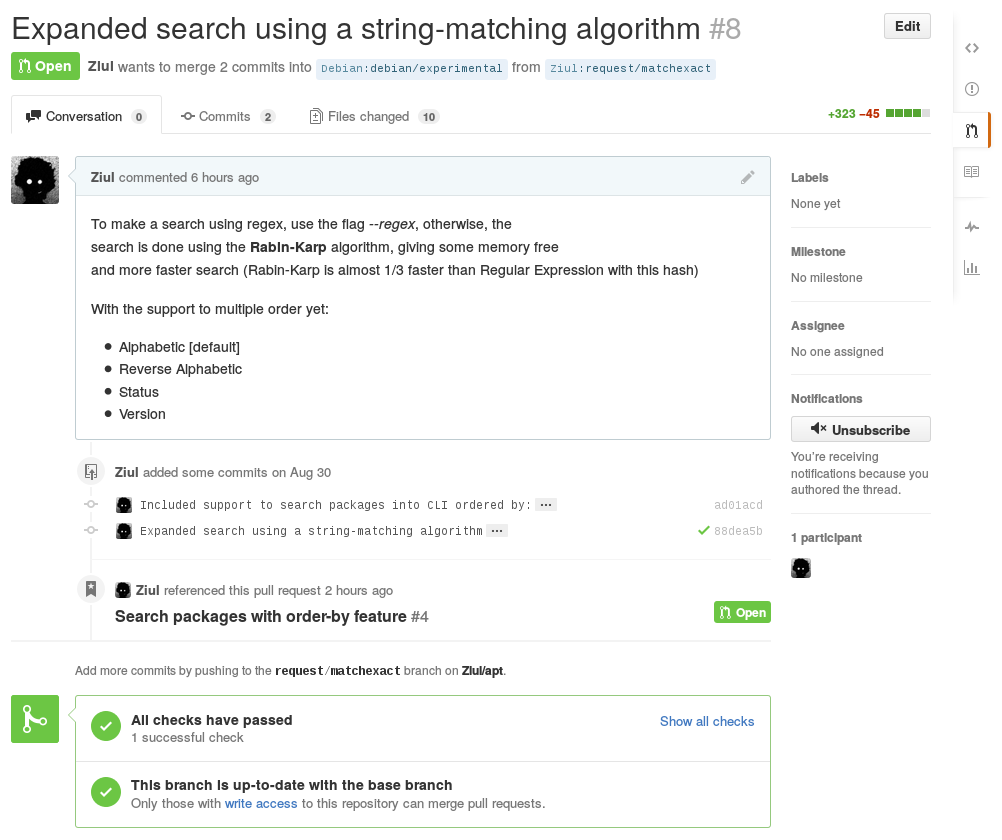
\includegraphics[width=0.95\textwidth]{figuras/pr2}
  \caption{Submissão do segundo \textit{merge request}}
  \label{fig:pr2_travisok}
\end{figure}

% section segunda_contribui_o (end)

\section{Terceira contribuição} % (fold)
\label{sec:terceira_contribui_o}

Esta contribuição corresponde ao objetivo principal deste trabalho: oferecer uma ferramenta de busca de pacotes o mais transparente possível quanto ao método de busca. Para atingir tal meta foram realizadas duas tarefas:

\begin{description}
	\item [Escolha entre expressões regulares ou não:] Mesmo oferecendo uma \textit{flag} para selecionar a busca com suporte a expressões regulares, era importante tornar o programa capaz de identificar se o parâmetro passado para a busca envolvia ou não uma \textit{regex} de fato. Isto é, se haviam caracteres especiais ou não no parâmetro de busca.
	\item [Inserir método de busca inexata:] Quando uma busca não obtiver nenhum resultado, a aplicação deveria executar a busca novamente utilizando um método de busca inexata e apontar os pacotes que poderiam estar relacionados ao parâmetro informado pelo usuário.
\end{description}

Para a primeira tarefa foi implementada uma função que verificava se, entre os parâmetros passados na busca, há caracteres especiais utilizados em expressões regulares. Estes caracteres eram {\code |\textbackslash\{\}[]():*+-\$?.\^{}}, porém os caracteres {\code .}, {\code :} e {\code -} costumam aparecer nos nomes dos pacotes os mesmos deveriam ser ignorados como indicativo de uso de expressões regulares.

\begin{lstlisting}[language=C++,label=regexidentify,caption={Identificação de Expressões Regulares}]
bool identify_regex(std::vector<std::string> input)
{
   /*
      not all characters can be included, as have
      packages with the chars .-:
   */
   std::string reserver_regex = "^$*+?()[]{}\\|";

   for(auto k:input)
      if( reserver_regex.find(k) == std::string::npos )
	 return true;
   return false;

}
\end{lstlisting}

O \autoref{regexidentify} apresenta uma solução para a identificação de caracteres que indicam o uso de expressões regulares nas buscas, verificando cada palavra em uma lista de \textit{strings} em busca dos caracteres citadas anteriormente. Caso algum caractere especial seja localizado, a função retorna verdadeiro.


Em seguida, foi verificada a \textit{flag} de uso de expressão regular ou caracteres reservados com o seguinte trecho de código:

\begin{lstlisting}[language=C++,basicstyle=\footnotesize\ttfamily,numbers=none]
if ((_config->FindB("APT::Cache::UsingRegex",false)) || identify_regex(args))
\end{lstlisting}

Caso a chamada acima seja verdadeira, as rotinas que compilam as expressões regulares serão executadas; caso contrário, o método de \nameref{ssub:rabin_karp} será executado para realizar a busca, visto este método ter apresentado melhor desempenho em relação ao método de \nameref{ssub:knuth_morris_pratt_}, dado que será melhor apresentando em maiores detalhes na \autoref{sec:algor_timos_de_string_matching_exatos}.


Finalizada esta etapa, o próximo, e último, passo foi identificar buscas onde nenhum pacote era localizado. Nestes casos, o algoritmo de \textit{\nameref{sec:leveinstein}} deveria ser utilizado para encontrar os pacotes que tivessem a menor diferença com o texto da pesquisa realizada. Essa chamada deveria ser realizada somente nos casos onde não houvesse o uso de expressões regulares.

Para realizar uma busca utilizando o modelo de \textit{Leveinstein} era necessário percorrer a lista de pacotes duas vezes. Na primeira vez eram pontuadas as distâncias dos nomes dos pacotes com os parâmetros de entrada da busca; na segunda vez os pacotes eram ordenados de acordo com sua pontuação. O \autoref{levisearchapt} apresenta a realização desta busca, percorrendo toda a lista de pacotes disponível ({\code bag}), e em seguida ordenando a saída.

\begin{lstlisting}[language=C++,label=levisearchapt,caption={Busca ordenada por distância de \textit{Levenshtein}}]
for(auto V:bag)
{

	// we want to list each package only once
	pkgCache::PkgIterator const P = V.ParentPkg();
	if (PkgsDone[P->ID] == true)
		continue;

	std::string PkgName = P.Name();
	pkgCache::DescIterator Desc = V.TranslatedDescription();
	pkgRecords::Parser &parser = records.Lookup(Desc.FileList());
	std::string const LongDesc = parser.LongDesc();

	for (auto arg:args)
	{
		int distance = levenshtein_distance(PkgName, arg);
		if ((distance >=0) && (distance <= (int)PkgName.length()/2 ))
		{
			PkgsDone[P->ID] = true;
			std::stringstream outs;
			ListSingleVersion(CacheFile, records, V, outs, format);
			outputVector.emplace_back(CacheFile, records, V, outs.str());
			outputVector.back().distance = distance;
		}
	}
}
std::sort(outputVector.begin(), outputVector.end(), OrderByDistance);
\end{lstlisting}

Devido ao fato das buscas inexatas consumirem mais recursos e de passarem duas vezes pela lista dos pacotes, elas foram delegadas apenas aos casos onde a busca não obtivesse nenhum resultado. O \autoref{calllevisearchapt} ilustra esta situação.

\begin{lstlisting}[language=C++,label=calllevisearchapt,caption={Chamada seletiva para buscas inexatas}]
if(outputVector.size() == 0)
{
	outputVector = SimilarSearch(bag,args);
	if(outputVector.size() > 10)
	outputVector.resize(10);
	std::cout << "None package fould. Maybe you are looking for one of those:" << std::endl;
}
\end{lstlisting}


Para o desenvolvimento desta contribuição, foi aproveitada a contribuição anterior, apenas atualizando a \textit{branch} com os novos \textit{commits}. Na \autoref{fig:pr3_travisok} podemos observar o mesmo \textit{merge request} requisitado para a segunda contribuição agora com o acréscimo do \textit{commit} {\code aae1adc}, onde todas as contribuições do terceiro grupo de contribuições deste trabalho foram agrupadas para simplificar a visualização e revisão do \textit{merge request}.

\begin{figure}[h]
  \centering
	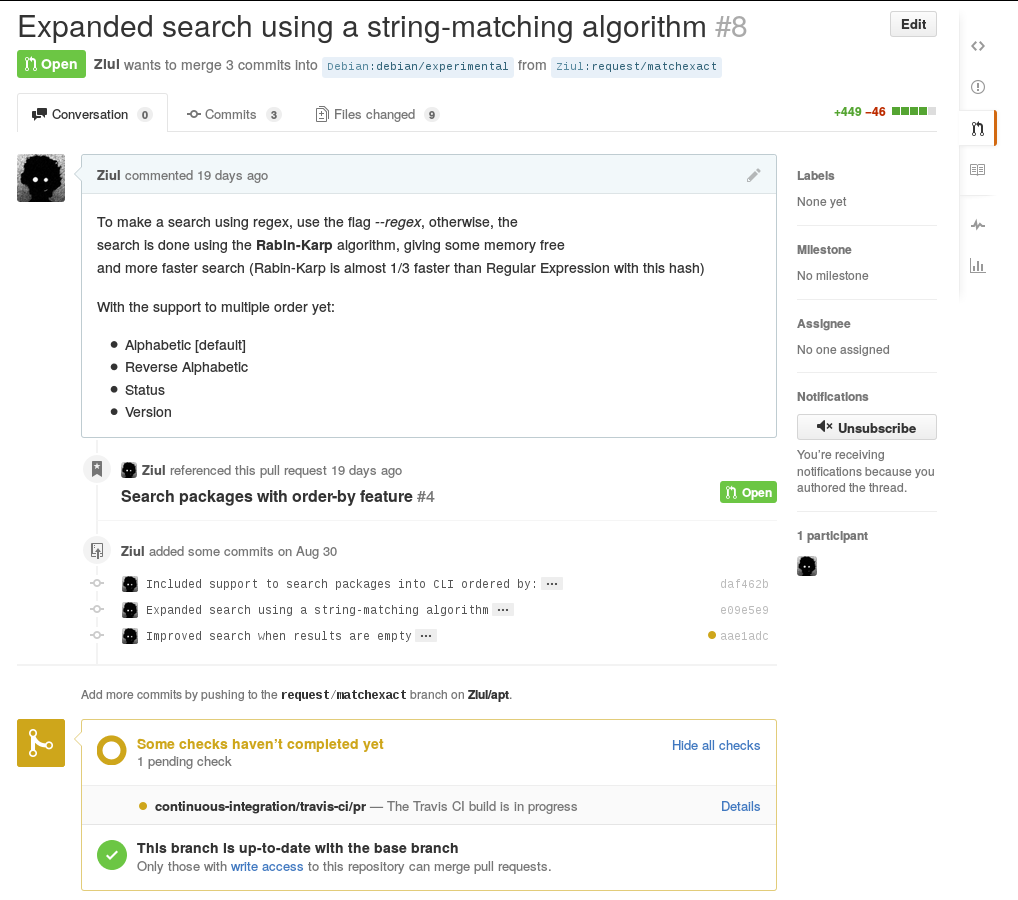
\includegraphics[width=0.95\textwidth]{figuras/pr3}
  \caption{Submissão do segundo \textit{merge request} atualizado com o conteúdo da terceira contribuição}
  \label{fig:pr3_travisok}
\end{figure}
% section terceira_contribui_o (end)
